\section{W10 - Inventory Management}
\subsection{Introduction}
\subsubsection{Water Consumption During the 2006 World Cup Championship}
\subsubsection{Visual Interpretation of Inventories}
\subsubsection{What other reasons are there for holding inventories?}
\subsubsection{Case Study: Leaving Everything Behind…}
\subsubsection{The Strategic Role of the Inventory: The Five Operations Performance Objectives}
\index{Operations!Performance Objectives}
Bsp: Zementfabrik, lange Anlaufzeit.\\
Ersatzteile, Kundennachfrage\\
cost -> Aktionen / Rabatte \\
\begin{itemize}
	\item Supporting \textbf{quality} objectives
	\item Supporting \textbf{speed} objectives
	\item Supporting \textbf{dependability} objectives
	\item Supporting \textbf{flexibility} objectives
	\item Supporting \textbf{cost} objectives
\end{itemize}
\subsubsection{Types of Inventory}
\begin{itemize}
	\item Buffer (NORDAL)
	\item Cycle
	\item De-coupling (Serielle Produktion (0.6*0.9))
	\item Anticipation (Gleichm\"assige Produktion, Absatz in kurzer frist, ex: Osterhasen)
	\item Pipeline (Lager w\"ahrend Transport)
\end{itemize}
\subsubsection{Disadvantages of Holding Inventory}
\begin{itemize}
	\item May become \textbf{obsolete} as alternatives become available
	\item Can be \textbf{damaged} or deteriorate
	\item Could be \textbf{totally lost},or be very expensive
	to retrieve
	\item Might be \textbf{hazardous} to store
	\item May need excessive \textbf{storage space} compared to its value
	\item If \textbf{duplicated} at different locations, it may be reordered at one
	location while excess inventory exists at others
	\item Involves high \textbf{administrative} and \textbf{insurance} costs
\end{itemize}
\subsubsection{Typical Inventory Profiles}
\subsubsection{The 3 Main Questions of Inventory Management}
\begin{itemize}
	\item \textbf{How much} should I order? (Q)
	\item \textbf{When} should I order? ($\frac{Q}{D}$)
	\item How should I \textbf{control the system}?
\end{itemize}
\subsection{Reordering Approach}
\subsubsection{Reducing the Reorder Quantity Reduces Stock While Increasing the Reorder Frequency}
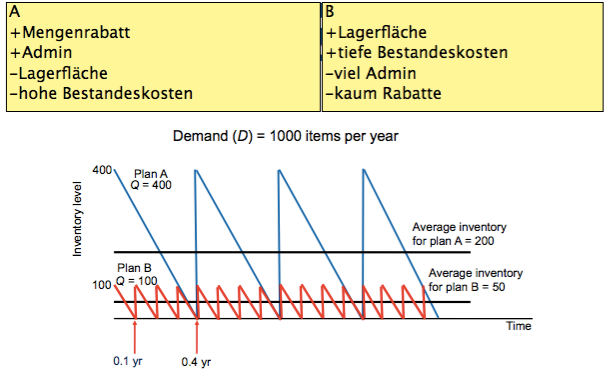
\includegraphics[width=1\textwidth]{W10/reducingreorder}
\subsubsection{Trade-Offs in Considering Optimal Quantity}
\subsubsection{EOQ\index{EOQ}: Economic Order Quantity (based on simplified assumptions)}
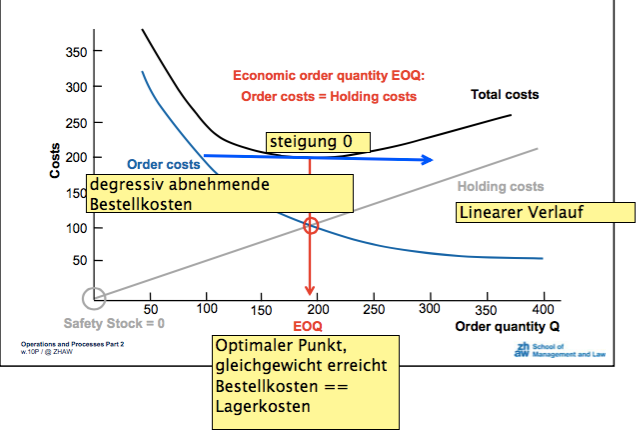
\includegraphics[width=1\textwidth]{W10/EOQ-simplyfied}
\subsubsection{How to Calculate the Economic Order Quantity }\label{EOQ}
\begin{center}
\begin{tabular}{|c|c|}
	\hline Holding Costs  & Order Costs \\ 
	\hline Working capital costs & Cost of placing an order \\
	Storage costs \& Price discount costs\\
	Obsolescence risk costs & \\
	\hline
\end{tabular}
\\\vspace{5 mm}
	\begin{tabular}{|r|l|}
		\hline EOQ  & Minimal total costs \\ 
		\hline Q  & Ordering quantity \\ 
		\hline $C_t$ & Total sourcing costs \\ 
		\hline $C_O$ & ordering costs per order\\ 
		\hline $D$ & Demand per Period$t_p$\\
		\hline $S$ & Safety Stock\\
		\hline $C_h$& Holding costs per unit ($t_p$)\\
		\hline
	\end{tabular}
	\\\vspace{5 mm}
	
	$C_h$ = $\frac{C_h\cdot Q}{2 + C_h \cdot S}$\\\vspace{2mm}
	$C_O$ = $\frac{C_O \cdot D}{Q}$\\\vspace{2mm}
	$C_t$ =  $C_h + C_O$\\\vspace{2mm}
	$EOQ = \frac{D \cdot C_t}{D \cdot Q} = 0$ \\\vspace{2 mm}
	$EOQ = \sqrt{\frac{2 \cdot C_O \cdot D}{C_h}}$ \\\vspace{2 mm}
	Order frequency = $\frac{D}{EOQ}$\\\vspace{2mm}
	Time between orders = $\frac{EOQ}{D}$\\\vspace{2mm}
	
\end{center}
\subsubsection{Exercise – determining the EOQ for our motors}

\subsubsection{The Total Costs Are Relatively Unaffected by Q}
\subsubsection{Reorder Point Method}
\subsubsection{Safety Stock Required to Cover Excessive Demand and/or Delivery Insecurity}
\subsubsection{How to Calculate the Safety Stock? Example: A Bar}
\subsubsection{Safety Stock and Remaining Risk: Demand and Delivery Lead Time are Statistic Distributions Frequency}
\subsubsection{Inventory Costs vs. Availability}
\subsection{Inventory Control}
\subsubsection{Pareto Curve for Stocked Items (ABC Analysis)}
\subsubsection{Inventory Classifications and Measures}
\subsubsection{Example: Pareto Distribution for a Pharmaceutical Co. A long tail of SKUs representing only a small part of the overall volume }
